% !TEX TS-program = XeLaTeX
\documentclass[10 pt, handout]{beamer}

% BEAMER SLIDES SETUP

\definecolor{burntorange}{rgb}{0.8, 0.33, 0.0}
\definecolor{darkcerulean}{rgb}{0.03, 0.27, 0.49}

\usecolortheme{rose}
\usefonttheme{professionalfonts}
\usefonttheme{serif}
\setbeamercolor{titlelike}{fg=burntorange}
\setbeamercolor{structure}{fg=darkgray}
\usepackage{hyperref}
\hypersetup{
    colorlinks=true,
    linkcolor=darkcerulean,
    citecolor=darkcerulean,
    filecolor=darkcerulean,
    urlcolor=darkcerulean,
}

% STYLE

\usepackage{float}
\usepackage{graphicx}
\graphicspath{ {./images/} }
\usepackage{subfig}
\usepackage{enumerate}
\usepackage[normalem]{ulem} % underlining
\usepackage{booktabs} % tables
\PassOptionsToPackage{table}{xcolor}% coloring tables

\AtBeginSection[]{ % section header slides
  \begin{frame}
  \vfill
  \centering
  \begin{beamercolorbox}[sep=8pt,center,shadow=true,rounded=true]{title}
    \usebeamerfont{title}\insertsectionhead\par%
  \end{beamercolorbox}
  \vfill
  \end{frame}
}

\setbeamertemplate{footline}[frame number] % slide numbers

% LANGUAGE + FONT
		    
\usepackage[english]{babel}
\usepackage[backend=biber,
                     style=unified]{biblatex}
\addbibresource{ref.bib}
\usepackage{fontspec}  
\usepackage{pifont}  
\setmainfont{Fira Sans}

% DRAWING

\usepackage{tikz}
\usetikzlibrary{matrix}

% LINGUISTICS 

%\usepackage{gb4e}
\usepackage{expex}
\usepackage[glossaries]{leipzig}
\makeglossaries
%\newleipzig {indef} {indef} {Indefinite}

\title{Контраст по глухости-звонкости в русской речи носителей лесного ненецкого}
\author{Александра Шикунова}
\institute{НИУ ВШЭ (Москва)}
\date{Молодые типологи, 24 ноября 2023}

\begin{document}

\begin{frame}
\titlepage
\end{frame}

%\begin{frame}{}
%    \tableofcontents
%\end{frame}

%			\section{}

\begin{frame}{Лесной ненецкий}

	\begin{enumerate}[$\gg$]
		\item Уральская семья > самодийская ветвь
		\item Ямало-Ненецкий АО, пуровский диалект
		\item Данные собраны в 2023 году в с. Харампур
	\end{enumerate}
	
	\begin{figure}[H]
		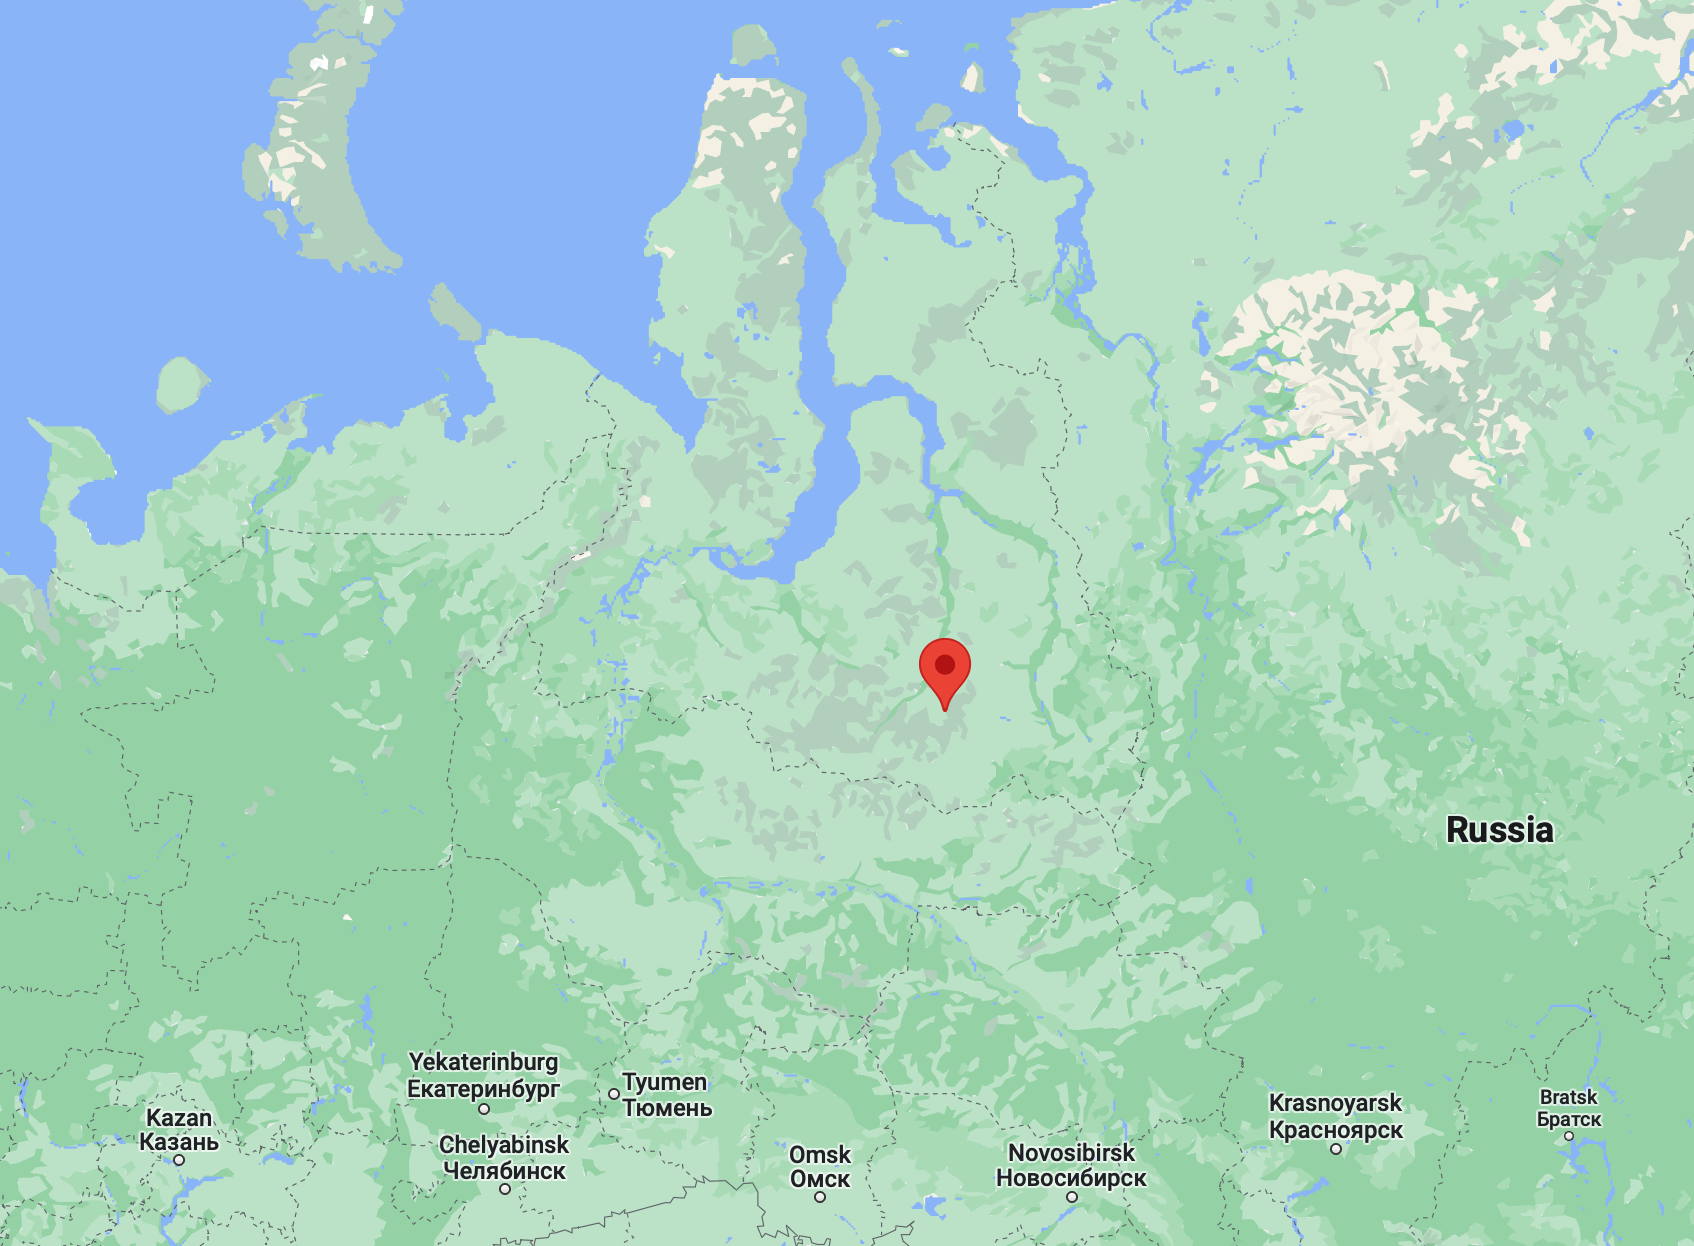
\includegraphics[width=.65\textwidth]{map}
	\end{figure}

\end{frame}

\begin{frame}{Звонкость-глухость в лесном ненецком}

	\begin{enumerate}[$\gg$]
		\item Контраста по звонкости-глухости нет (не редкость, характерно для примерно трети языков; \cite{wals-4})
		\item Контакт с русским языком, где контраст есть (редкость; \cite{broselow2018})
		\item В русском языке контраст есть
	\end{enumerate}
	
\begin{table}[H]
\begin{tabular}{cccc}
p pˊ & t č  & k kˊ & ʰ/ʔ \\
m mˊ & n nˊ & ŋ ŋˊ &     \\
s sˊ & x xˊ &      &     \\
λ λˊ &      &      &     \\
w wˊ & l lˊ &      &     \\
dˊ   &      &      &    
\end{tabular}
\caption{Инвентарь согласных в ЛН}
\end{table}

	\vfill
	Как звучит лесной ненецкий акцент в русском?
	
\end{frame}

\begin{frame}{Звонкость-глухость в лесном ненецком}

	\begin{enumerate}[$\gg$]
		\item ``Тотальное оглушение''
		\item Происходит не всегда, но заметно часто
	\end{enumerate}
	
	\pex
		\a \emph{декабрь} {[текапрь]}
		\a \emph{может} {[мошет]}
		\a \emph{обычай} {[опычай]}
		\a \emph{замуж} {[самуш]}
	\xe
	
\end{frame}

\begin{frame}[fragile]{Звонкость-глухость в L2}

	О нейтрализации контраста по звонкости-глухости установлены некоторые универсалии (\cite{eckman1977} et seq.)

	\begin{enumerate}[$\gg$]
		\item Наименее маркированным вариантом является глухой
		\item Позиции выстраиваются в иерархию маркированности относительно контраста по звонкости-глухости:
	\end{enumerate}
		
%	\ex финальная позиция > нефинальная позиция\\
%		(маркированная) > (немаркированная)
%	\xe
	
	\ex Иерархия позиций, где может сохранятся контраст
\begin{tikzpicture}
\matrix [matrix of nodes, row sep=.1em,
column sep={6.7em,between origins}]
{
финальная позиция & > & нефинальная позиция\\
(маркированная) & {} & (немаркированная) \\
};
\end{tikzpicture}
	\xe

\end{frame}

\begin{frame}{Гипотезы и ожидания}

	От L2-русского у носителей лесного ненецкого мы ожидаем:

	\begin{enumerate}[$\gg$]
		\item \textbf{Нейтрализации контраста}\\
			$\Rightarrow$ VOT русских глухих взрывных не отличается от звонких в их речи\\
			$\Rightarrow$ Шумные согласные не отличаются по звонкости-глухости
		\item \textbf{Нейтрализации контраста в сторону глухости}\\
			$\Rightarrow$ VOT взрывных согласных -- положительное\\
			$\Rightarrow$ Шумные согласные не озвучены
	\end{enumerate}

\end{frame}

	\section{Данные}

\begin{frame}{Данные}

	\begin{enumerate}[$\gg$]
		\item Два социолингвистических интервью с носительницами лесного ненецкого как родного
		\item Русский выучили в школе-интернате
		\item Свободное порождение русской речи
		\item Размечено несколько слоев
			\begin{enumerate}[$\cdot$]
				\item слова
				\item сегменты
				\item взрыв (точечный слой; для взрывных)
				\item озвученность (совпадает по интервалам с сегментами)
			\end{enumerate}
		\item Контексты: \#\_V, V\_V, V\_\#
	\end{enumerate}

\end{frame}

\begin{frame}{Статистический анализ}

	\textbf{Гипотеза 1}: VOT русских глухих взрывных не отличается от звонких в речи носителей ЛН
	\vfill
	
\begin{tabular}{lrrrl}
\toprule
\textbf{Сегмент} &  \textbf{VOT глухого} &  \textbf{VOT звонкого} &       \textbf{p} & \textbf{Значимость} \\
\midrule
 п vs б &      37.6 &      30.2 & 0.28374 &          нет \\
 т vs д &      45.7 &      43.6 & 0.72214 &          нет \\
 к vs г &      54.2 &      28.2 & 0.00825 &         да \\
\bottomrule
\end{tabular}

	\vfill
	\begin{enumerate}[$\gg$]
		\item Судя по t-тесту с двусторонней альтернативой, значимой разницы между звонкими и глухими нет
		\item Кроме к/г: /г/ имеет значимо меньший VOT, тем не менее, среднее положительно
	\end{enumerate}

\end{frame}

\begin{frame}{Статистический анализ}

	\textbf{Гипотеза 2}: Шумные согласные не отличаются по звонкости-глухости
	\vfill
	
\begin{tabular}{lrrr}
\toprule
\textbf{Сегмент} &  \textbf{Длительность} &  \textbf{Доля звонких} & \textbf{Кол.-во наблюдений}\\
\midrule
ф       &     0.096 &   0.000 &     10 \\
\textbf{в}       &     0.077 &   \textbf{0.954} &    219 \\
ш       &     0.122 &   0.000 &     69 \\
ж       &     0.103 &   0.083 &    168 \\
с       &     0.105 &   0.006 &    166 \\
з       &     0.113 &   0.140 &    107 \\
\bottomrule
\end{tabular}

	\vfill

	\begin{enumerate}[$\gg$]
		\item По частотности озвученности выделяется только /в/
		\item /в/ практически всегда звонкое
	\end{enumerate}

\end{frame}

\begin{frame}{Статистический анализ}

	Укладываются ли взрывные в L2-русском лесных ненцев в рамки русских глухих взрывных?
	\vfill
	
\begin{tabular}{lrrrlr}
\toprule
\textbf{Сегмент} &  \textbf{VOT} &  \textbf{VOT (ож.)} &       \textbf{p} & \textbf{Значимость}\\
\midrule
      п &      37.7 &      18.0 & 0.00001 &         да \\
      б &      27.7 &     -70.0 & 0.00000 &         да \\
      т &      41.6 &      20.0 & 0.00040 &         да \\
      д &      39.4 &     -75.0 & 0.00000 &         да \\
      к &      51.6 &      38.0 & 0.02976 &         да \\
      г &      25.9 &     -78.0 & 0.00000 &         да \\
\bottomrule
\end{tabular}

	\vfill
	\begin{enumerate}[$\gg$]
		\item Укладываются нет все, но у всех VOT больше, чем в русском, то есть ненецкие взрывные глуше
	\end{enumerate}

\end{frame}

\begin{frame}{Статистический анализ}

	Есть ли разница между конечным и неконечным контекстами относительно оглушения?
	\vfill

\begin{tabular}{lrrrl}
\toprule
\textbf{Сегмент} &  \textbf{VOT фин.} &  \textbf{VOT нефин.} &       \textbf{p} & \textbf{Значимость} \\
\midrule
 п vs б &      37.7 &      27.7 & 0.18388 &          нет \\
 т vs д &      41.6 &      39.4 & 0.73299 &          нет \\
 к vs г &      51.6 &      25.9 & 0.03135 &         да \\
\bottomrule
\end{tabular}

	\vfill
	\begin{enumerate}[$\gg$]
		\item Для тех случаев, когда данных достаточно для сравнения, видно, что разницы нет
	\end{enumerate}

\end{frame}

\begin{frame}{Промежуточный итог}

	\begin{enumerate}[$\gg$]
		\item Данные спонтанной речи показывают, что оглушение есть
		\item По крайней мере, в большинстве случаев
		\item Влияния контекста не замечено
		\item /в/ выбивается из общей картины: он не глухой
	\end{enumerate}

\end{frame}

	\section{Интерпретация}

\begin{frame}{Оглушение}

	\begin{enumerate}[$\gg$]
		\item Как и ожидается, нейтрализация контраста по глухости-звонкости происходит в сторону менее маркированного варианта
		\item Между финальной и нефинальной позициями разницы нет
		\item В русском в финальной позиции контраст уже нейтрализован
		\item В ненецком нет контраста и в нефинальной позиции -- полная нейтрализация
	\end{enumerate}

\end{frame}

\begin{frame}{Особый статус /в/}

	Шумные согласные тоже подвержены оглушению, но /в/ всегда звонкий. Причина 1:

	\begin{enumerate}[$\gg$]
		\item /в/ ассоциирован с /w/, который в ЛН является звонким аппроксимантом
		\item Все остальные шумные и взрывные тоже не противопоставлены по звонкости-глухости, но являются глухими
		\item Глухого /f/ в ЛН нет; ``чужие'' звуки в L2 усваиваются точнее \parencite{flege1987}
	\end{enumerate}

\end{frame}

\begin{frame}{Особый статус /в/}

	Шумные согласные тоже подвержены оглушению, но /в/ всегда звонкий. Причина 2:

	\begin{enumerate}[$\gg$]
		\item /в/ -- особая фонема в русском
		\item /в/ может оглушаться до /ф/ на конце слов
		
		\pex 
			\a \emph{корова} [в] -- \emph{коров} [ф]
			\a \emph{дорога} [г] -- \emph{дорог} [к]
		\xe

		\item Шумные и взрывные в русском вызывают регрессивную ассимиляцию по звонкости-глухости
		
		\pex 
			\a \emph{делал} [д] -- \emph{сделал} [зд]
			\a \emph{танцевал} [т] -- \emph{станцевал} [ст]
		\xe
	\end{enumerate}
		
\end{frame}

\begin{frame}{Особый статус /в/}

	\begin{enumerate}[$\gg$]
		\item Кроме /в/: он ведет себя как сонорный
		\pex 
			\a \emph{вёл} [в] -- \emph{свёл} [св]
			\a \emph{мял} [м] -- \emph{смял} [см]
		\xe
		\item Возможное основание для того, чтобы /в/ воспринимался носителями ЛН как сонорный и, следовательно, звонкий
	\end{enumerate}

\end{frame}

\begin{frame}{Планы на будущее}

\centering
\begin{tabular}{lr}
\toprule
\textbf{Сегмент} &  \textbf{Кол.-во} \\
\midrule
т       &    525 \\
д       &    327 \\
к       &    217 \\
п       &    212 \\
б       &    141 \\
г       &     86 \\
\bottomrule
\end{tabular}

\vfill

\begin{tabular}{lr}
\toprule
\textbf{Контекст} &  \textbf{Кол.-во} \\
\midrule
начальный &     1670 \\
средний  &      489 \\
финальный   &       88 \\
\bottomrule
\end{tabular}

\end{frame}

\begin{frame}{Планы на будущее}

	\begin{enumerate}[$\gg$]
		\item Баланса в выборке нет: смещение в сторону зубных и начальных
		\item Экспериментальный дизайн, включающий сбалансированное распределение контекстов и сегментов -- надёжнее
		\item Исследование восприятия контраста /в/--/ф/ по сравнению с другими необходимо, чтобы обосновать влияние фонологического поведения /в/ в русском на его звонкость %в речи лесных ненцев
	\end{enumerate}

\end{frame}

\begin{frame}{Благодарности}

				\begin{enumerate}[\ding{170}]
					\item Марии Аристовой и Алексею Козлову за социолингвистические интервью
					\item Каролине Берзиной за разметку
				\end{enumerate}

\end{frame}

	\section{Приложение}

\begin{frame}{Средние VOT смычных}

\begin{tabular}{lrrr}
\toprule
\textbf{Сегмент} &  \textbf{Кол.-во} &   \textbf{Среднее} &    \textbf{Ст. отклонение} \\
\midrule
п       &    212 &  0.045 &  0.121 \\
б       &    141 &  0.022 &  0.116 \\
т       &    525 &  0.033 &  0.217 \\
д       &    327 &  0.040 &  0.212 \\
к       &    217 &  0.055 &  0.299 \\
г       &     86 & -0.015 &  0.294 \\
\bottomrule
\end{tabular}

\end{frame}

\begin{frame}[allowframebreaks]
\frametitle{References}
%\bibliography{ref}
\printbibliography
\end{frame}

\end{document}